% =============================================================================
% PNDR Survey - Systematic Literature Review
% =============================================================================
% Article: Avaliação dos Instrumentos da PNDR: Uma Revisão Sistemática
%          da Literatura Empírica (2005--2026)
%
% Author:  Hermelino Nepomuceno de Souza
% =============================================================================

\documentclass[
12pt,             % Tamanho da fonte
a4paper,          % Tamanho da folha A4
article,          % Modo artigo (sem chapters)
oneside,          % Impressão em apenas uma face
english,          % Hifenizações em inglês
brazil            % Último idioma é o idioma padrão
]{abntex2}

% --- Encoding ---
\usepackage{cmap}           % Gera CMap correto no PDF (acentos copy-paste)
\usepackage[utf8]{inputenc}
\usepackage[T1]{fontenc}

% --- Page Layout ---
\usepackage[top=2.5cm, bottom=2.5cm, left=3cm, right=2.5cm]{geometry}
\OnehalfSpacing

% --- Fonts ---
\usepackage{lmodern}

% --- Math ---
\usepackage{amsmath,amssymb}

% --- Tables (booktabs e tabularx já carregados por memoir/abntex2) ---
\usepackage{longtable}
\usepackage{multirow}
\usepackage{afterpage}  % Para posicionamento de tabelas
\usepackage{pdflscape}  % Tabelas em formato paisagem

% --- Figures ---
\usepackage{graphicx}
\graphicspath{{../figures/}}
\usepackage{float}

% --- Citations (ABNT) ---
\usepackage[alf, abnt-emphasize=bf, recuo=0cm, abnt-etal-cite=2, abnt-etal-list=0, abnt-etal-text=it]{abntex2cite}

% --- Hyperlinks ---
\hypersetup{
    colorlinks=true,
    linkcolor=blue,
    citecolor=blue,
    urlcolor=blue
}

% --- Misc ---
\usepackage{enumerate}
\usepackage{enumitem}
\usepackage{caption}
\usepackage{subcaption}
\usepackage{indentfirst}
\usepackage{../docs/prisma-flow-diagram}

% --- Fonte/Nota alinhadas à esquerda (override abntex2) ---
\renewcommand{\fonte}[1]{%
  \begin{flushleft}
    \footnotesize Fonte: #1
  \end{flushleft}
}

% --- Contador e nome para Quadros (ABNT) ---
\newcounter{quadro}
\renewcommand{\thequadro}{\arabic{quadro}}
\newcommand{\quadroname}{Quadro}

% =============================================================================
% --- Metadados abnTeX2 ---
\titulo{Avaliação dos Instrumentos da PNDR: Uma Revisão Sistemática da Literatura Empírica (2005--2026)}
\tituloestrangeiro{}

\autor{
    Hermelino Nepomuceno de Souza\thanks{CAEN/UFC.} \and
    Guilherme Diniz Irffi\thanks{CAEN/UFC.} \and
    Diego Rafael Fonseca Carneiro\thanks{CAEN/UFC.} \and
    Felipe de Sousa Bastos\thanks{CAEN/UFC.}
}

\data{\today}

% =============================================================================
\begin{document}

\maketitle
\textual

% --- Abstract ---
\begin{abstract}
Esta revisão sistemática mapeia e sintetiza a literatura empírica que avalia os efeitos dos instrumentos da Política Nacional de Desenvolvimento Regional (PNDR) --- Fundos Constitucionais de Financiamento, Fundos de Desenvolvimento Regional e Incentivos Fiscais --- sobre indicadores socioeconômicos locais. Seguindo o protocolo PRISMA 2020, a busca foi conduzida em cinco bases de dados acadêmicas e resultou na seleção de 44 estudos publicados entre 2005 e 2026. Os principais achados indicam: (i)~expressiva assimetria de evidências, com 38 dos 44 estudos concentrados nos Fundos Constitucionais; (ii)~maior convergência nos efeitos sobre o emprego formal do que sobre o PIB \textit{per capita}; (iii)~eficácia dos Fundos Constitucionais condicionada ao nível inicial de renda dos municípios, com efeitos positivos em faixas intermediárias e nulos em municípios de baixa renda; (iv)~indícios de impacto expressivo dos Fundos de Desenvolvimento (21--24\% no PIB \textit{per capita}), porém com base empírica restrita; e (v)~ausência de ganhos de produtividade associados à geração de empregos. As lacunas prioritárias incluem a inexistência de avaliações dedicadas ao FDA, FDCO e incentivos da SUDAM, a escassez de estudos multi-instrumento e a sub-representação de métodos quase experimentais com maior poder de identificação causal.

    \noindent\textbf{Palavras-chave:} PNDR; Revisão Sistemática; Fundos Constitucionais; Fundos de Desenvolvimento; Incentivos Fiscais.

    \vspace{0.5cm}
    \noindent\textbf{JEL:} R11; R58; H50; O18.
\end{abstract}

\newpage

% =============================================================================
% SECTIONS
% =============================================================================

\section{Introdução}
\label{sec:introducao}
% Arquivo: latex/1-introducao.tex
% Seção 1: Introdução

A desigualdade regional constitui um dos traços estruturais mais persistentes da economia brasileira. As regiões Norte e Nordeste concentram historicamente os piores indicadores de renda, educação e infraestrutura, enquanto Sul e Sudeste respondem pela maior parcela do produto nacional \cite{Ferreira1995,Silveira2011}. Embora estudos identifiquem processo de convergência dos níveis regionais de renda ao longo das últimas décadas, a velocidade é insuficiente para eliminar as disparidades em horizonte razoável: \citeonline{Cruz2014} estimam que, mantido o ritmo de crescimento diferencial observado, o Nordeste levaria cinquenta anos para atingir 75\% do PIB \textit{per capita} nacional. Dados recentes indicam que cerca de 90\% dos municípios das áreas de atuação da SUDAM, SUDENE e SUDECO classificados na faixa inferior de renda em 2002 permaneciam na mesma condição em 2021, evidenciando elevada persistência do baixo desenvolvimento \cite{Portugal2024}.

Nesse contexto, a Política Nacional de Desenvolvimento Regional (PNDR), instituída pelo Decreto nº 6.047/2007 e reformulada em 2019 e 2024, opera por meio de três instrumentos de financiamento voltados às regiões Norte, Nordeste e Centro-Oeste: os Fundos Constitucionais de Financiamento (FNE, FNO e FCO), que oferecem crédito subsidiado aos setores produtivos locais; os Fundos de Desenvolvimento Regional (FDNE, FDA e FDCO), direcionados a projetos estruturantes de grande porte; e os Incentivos Fiscais administrados pela SUDAM e SUDENE, que operam via renúncia tributária para atrair investimentos privados \cite{Portugal2020}. O volume de recursos públicos mobilizado por esses instrumentos é expressivo: no período 2002--2021, as aplicações acumuladas dos Fundos Constitucionais totalizaram cerca de R\$ 549 bilhões (valores de 2020), os Fundos de Desenvolvimento liberaram aproximadamente R\$ 18,9 bilhões em financiamentos, e os Incentivos Fiscais da SUDAM e SUDENE responderam por R\$ 126 bilhões em gastos tributários entre 2015 e 2024 \cite{Portugal2024}.

Apesar da longevidade dos programas --- os Fundos Constitucionais operam ininterruptamente desde 1989 e os Incentivos Fiscais desde a década de 1960 --- e do volume substancial de recursos envolvidos, a persistência das disparidades regionais torna imprescindível a avaliação rigorosa da eficácia desses instrumentos. A adoção de práticas sistemáticas de monitoramento e avaliação é condição necessária para verificar se os objetivos da política estão sendo alcançados, identificar falhas de desenho e fundamentar ajustes na alocação dos recursos \cite{Lima2025}. No caso de políticas de desenvolvimento regional, a avaliação enfrenta desafios metodológicos específicos: a dificuldade de construir grupos contrafactuais adequados, a multiplicidade de indicadores de resultado, a presença de efeitos de transbordamento espacial e a defasagem temporal entre a intervenção e a maturação dos seus efeitos \cite{Oecd2025}.

Essas dificuldades fazem com que métodos experimentais randomizados sejam raramente factíveis na avaliação de políticas regionais, levando os pesquisadores a recorrer a métodos de painel com efeitos fixos, modelos espaciais, técnicas de \textit{matching} e desenhos quase experimentais como diferenças em diferenças, regressão com descontinuidade e controle sintético. Nas últimas duas décadas, uma literatura empírica crescente buscou estimar os efeitos dos instrumentos da PNDR sobre indicadores socioeconômicos locais empregando essas abordagens. Os estudos, contudo, encontram-se dispersos em periódicos nacionais e internacionais, \textit{working papers}, textos para discussão e anais de congressos, dificultando uma visão integrada do estado das evidências.

Revisões prévias da literatura puderam identificar padrões importantes nessa produção, embora com escopos parciais. \citeonline{Resende2013} realizou levantamento da literatura de avaliação de políticas regionais no Brasil e apontou relativa escassez de estudos empíricos no período 2000--2009, com apenas duas avaliações de impacto identificadas. \citeonline{Portugal2017} analisou estudos realizados entre 2005 e 2016 e constatou que os Fundos Constitucionais são os instrumentos mais investigados, com evidências de impacto positivo sobre emprego e massa salarial, mas com resultados divergentes sobre o PIB \textit{per capita}. \citeonline{CarneiroCambota2018} sintetizaram evidências empíricas específicas do FNE, concluindo por efeitos geralmente positivos, porém heterogêneos entre setores e mais pronunciados para micro e pequenas empresas. \citeonline{Shirasu2023} revisaram estudos sobre incentivos fiscais, mas relataram pouca aplicação ao contexto específico da PNDR. Nenhuma dessas revisões, contudo, adotou protocolo sistemático de busca e seleção, tampouco abrangeu simultaneamente os três instrumentos em horizonte temporal amplo.

A pergunta de pesquisa que orienta este artigo é: qual é o estado das evidências empíricas sobre os efeitos dos Fundos Constitucionais, Fundos de Desenvolvimento e Incentivos Fiscais da PNDR sobre indicadores socioeconômicos locais --- em particular PIB \textit{per capita}, emprego formal e salário médio --- no período de 2005 a 2026? O artigo contribui para preencher a lacuna identificada ao conduzir uma revisão sistemática conforme o protocolo PRISMA 2020 \cite{Page2021}, com busca em cinco bases de dados acadêmicas (Scopus, SciELO, Catálogo de Teses e Dissertações da CAPES, EconPapers/RePEc e Encontros da ANPEC) e seleção de 34 estudos empíricos.

Para além da síntese comparativa dos resultados por instrumento e abordagem metodológica, o artigo incorpora inovações procedimentais que o diferenciam das revisões anteriores: (i)~processo de deduplicação em quatro fases (DOI exato, título por similaridade \textit{fuzzy}, PDF idêntico e verificação manual de textos para discussão e versões de congresso); (ii)~classificação assistida por modelo de linguagem (Gemini 2.0 Flash), em três estágios de análise, com revisão manual subsequente; e (iii)~cálculo de índice de citação cruzada entre os estudos selecionados, que permite identificar os trabalhos mais influentes dentro do campo e mapear a rede de referências da literatura.

Os principais resultados da revisão indicam: (i)~expressiva assimetria de evidências, com 28 dos 34 estudos concentrados nos Fundos Constitucionais e predominância do FNE; (ii)~maior convergência nas estimativas de impacto sobre o emprego formal do que sobre o PIB \textit{per capita}; (iii)~eficácia dos Fundos Constitucionais condicionada ao nível inicial de renda dos municípios, com efeitos positivos em faixas intermediárias de desenvolvimento e nulos em municípios de baixa renda; (iv)~indícios de impacto expressivo dos Fundos de Desenvolvimento sobre o PIB \textit{per capita} (entre 19\% e 24\%), porém com base empírica ainda restrita; e (v)~ausência de ganhos de produtividade associados à geração de empregos nos instrumentos avaliados.

O restante do artigo organiza-se da seguinte forma: a Seção~\ref{sec:politica_regional} contextualiza a política regional no Brasil e descreve o funcionamento dos três instrumentos; a Seção~\ref{sec:metodo} apresenta a estratégia metodológica da revisão sistemática; a Seção~\ref{sec:resultados} discute os resultados organizados por instrumento; e a Seção~\ref{sec:consideracoes} apresenta as considerações finais, incluindo implicações para o desenho da política e lacunas prioritárias para a agenda de pesquisa.


\section{Política Regional no Brasil}
\label{sec:politica_regional}
% Arquivo: latex/2-politica-regional.tex
% Seção 2: Política Regional no Brasil
% Artigo: Avaliação dos Instrumentos da PNDR
% Gerado em: 2026-03-02


As regiões Norte e Nordeste concentram cerca de 36\% da população do país, mas respondem por apenas 20\% do PIB nacional\footnote{IBGE, Contas Regionais do Brasil, 2021. Norte: 6,3\%; Nordeste: 13,8\% do PIB.}. O Nordeste, em particular, registra o menor PIB \textit{per capita} entre as macrorregiões, com participação média de 13,6\% no produto nacional no período 2002--2020, além de uma base industrial reduzida (9,2\% do valor adicionado, ante 13,4\% da média nacional) e elevada concentração da atividade econômica em três estados --- Bahia, Pernambuco e Ceará ---, que respondem por 62,8\% do PIB regional \cite{Trece2023}.

Diante da magnitude e da persistência dessas disparidades, o governo federal  tem executado ao longo de mais de seis décadas variados instrumentos de política regional voltados à promoção do desenvolvimento das regiões menos dinâmicas. A trajetória institucional desses instrumentos, dos primeiros esforços na década de 1950 à atual configuração da Política Nacional de Desenvolvimento Regional, é brevemente apresentada a seguir.

\subsection{Origens e evolução histórica da política regional}
\label{subsec:origens-evolucao}

A região Nordeste foi a primeira macrorregião a receber atenção especial do governo central em razão de suas disparidades elevadas de renda e desenvolvimento em relação ao restante do país. Diagnóstico feito ao fim da década de 1950 pelo Grupo de Trabalho para o Desenvolvimento do Nordeste~\cite{GTDN1959} aponta a região como a mais atrasada do país, com baixo nível de renda, elevada concentração fundiária, infraestrutura precária e economia baseada na monocultura de exportação.

Para \citeonline{Moreira2014}, a problemática da desigualdade regional surge da divisão territorial do trabalho resultante do processo de industrialização nacional ocorrido entre 1880 e 1930, e intensificando-se após 1950. O contraste entre as estruturas produtivas durante boa parte do século XX (o Nordeste açucareiro/pecuário-algodoeiro e o Centro-Sul cafeeiro/industrial) marcou profundamente as relações de produção entre as principais regiões do país. Para a linha teórico-estruturalista de \citeonline{Prebisch1949} e \citeonline{Furtado2009}, essas desigualdades decorrem da reprodução, em âmbito nacional, da relação de dependência centro-periferia caracterizada por uma metrópole industrializada produzindo bens de alto valor agregado versus periferia produtora de matérias-primas.

Os primeiros esforços sistemáticos de política de desenvolvimento regional no Brasil remontam às décadas de 1950 e 1960, com a criação da Superintendência de Valorização Econômica da Amazônia (SPVEA), pela Lei nº 1.806/1953, e da SUDENE, pela Lei nº 3.692/1959 \cite{Silva2014,Portugal2020}. A SUDENE, instituída sob a visão teórica de \citeonline{Furtado2009}, tornou-se central no esforço do governo federal em superar o atraso relativo da região. O diagnóstico apontava para a industrialização como o caminho para o desenvolvimento regional e a participação do Estado na economia era vista como fundamental.

Ao final dos anos 50, o arranjo federativo existente permitia certa autonomia aos orgãos regionais de desenvolvimento, que atuavam em cooperação com os governos estaduais \cite{Bercovici2003}, em especial a SUDENE. A forma principal de atuação não era a ação direta do Estado, mas a concessão de subsídios fiscais e financeiros a empresas que realizassem investimentos produtivos nas regiões prioritárias. 

Durante o Regime Militar (1964--1985), o modelo foi estendido a outras regiões: a SPVEA deu lugar à SUDAM, e a SUDECO substituiu a antiga Fundação Brasil-Central. Apesar do avanço institucional, o que se viu no período foi a centralização do planejamento estatal, submetendo as superintendências aos objetivos dos planos nacionais de desenvolvimento e esvaziando sua autonomia \cite{Silva2014}. 

Durante as décadas seguintes as políticas de cunho regional foram esvaziadas, o contexto de crise fiscal do Estado e a transição para um modelo estatal regulador reduziram drasticamente a capacidade de financiamento das políticas regionais. Em 2001, as superintendências SUDAM e SUDENE foram extintas e substituídas por agências de desenvolvimento (ADA e ADENE), que passam a atuar mais como executoras, e não formuladoras, de políticas \cite{Portugal2020}.

\subsection{Política Nacional de Desenvolvimento Regional (PNDR)}
\label{subsec:pndr}

A Constituição Federal de 1988 estabeleceu as bases para a retomada da questão regional ao inserir a redução das desigualdades regionais como princípio fundamental (Art. 3º, inciso III) e ao destinar 3\% da arrecadação de IR e IPI a programas de financiamento produtivo de caráter regional. São criados os Fundos Constitucionais de Financiamento --- FNE, FNO e FCO --- com o objetivo de direcionar crédito subsidiado aos setores produtivos locais. Esses fundos tornariam-se a maior fonte de financiamento de políticas regionais.

Em 2007, por meio do Decreto nº 6.047, é instituída a PNDR, com o objetivo expresso de reduzir as desigualdades socioeconômicas entre as regiões brasileiras e promover a equidade no acesso a oportunidades de desenvolvimento. A política parte do diagnóstico de que a desigualdade resulta da dinâmica assimétrica do crescimento capitalista e exige abordagem em múltiplas escalas, reconhecendo diferentes dinâmicas sub-regionais \cite{Brasil2006}. Como instrumentos de ação, a mesma lei institui o Fundos de Desenvolvimento da Amazônia (FDA) e o Fundo de Desenvolvimento do Nordeste (FDNE), voltados ao financiamento de investimentos privados de grande porte.

Ainda em 2007, são reestabelecidas as superintendências regionais SUDAM e SUDENE, por meio das Leis Complementares nº 124/2007 e nº 125/2007, respectivamente. E pouco depois pe instituída a SUDECO, pela LC nº 129/2009. A PNDR passou a contar com três modalidades operacionais de financiamento: Fundos Constitucionais, Fundos de Desenvolvimento e os incentivos fiscais administrados por SUDENE e SUDAM. Um instrumento adicional --- o Fundo Nacional de Desenvolvimento Regional (FNDR) --- foi prevista, mas somente regulamentado em 2023 (EC nº 132/2023).

Para orientar a alocação de recursos, foi estabelecida uma tipologia de áreas prioritárias definidas a partir do rendimento médio por habitante e da variação do PIB \textit{per capita}, classificando os municípios como baixa renda, estagnados, dinâmicos ou alta renda. Essa classificação é utilizada para definir os critérios de elegibilidade aos benefícios e as condições de financiamento, buscando direcionar os recursos para as regiões mais necessitadas.

Em 2019, por meio do Decreto nº 9.810, formaliza-se a PNDR II, cujos objetivos centrais incluem a convergência dos níveis de desenvolvimento entre e intrarregiões e o estímulo à competitividade em áreas de declínio econômico. O novo texto trás avanços, em especial no aspecto de governança da política, mas os instrumentos de financiamento permanecerem inalterados.

Apesar dos avanços institucionais, \citeonline{Portugal2020} avaliam que a política de modo geral tem falhado em seus objetivos, devido à: (i) inexistência de marco normativo com maiores vínculos jurídicos (como uma lei, em lugar de decreto); (ii) baixa colaboração e coordenação entre entes federativos e ministérios; (iii) ausência da questão regional na agenda de prioridades do governo. \citeonline{Coelho2015} reforça que as instituições regionais não contaram com instrumentos efetivos para enfrentar as desigualdades regionais e lembra que a operacionalização da política foi comprometida pela tardia aprovação do FNDR.

\subsection{Fundos Constitucionais de Financiamento}
\label{subsec:fcs}

Os fundos constitucionais visam a oferta de micro-crédito produtivo a taxas de juros subsidiadas e prazos mais longos, incentivando a abertura de novos negócios e a geração de renda nas regiões prioritárias. A legislação que regulamenta os FCs (Lei nº 7.827/1989) também estipula tratamento preferencial a micro e pequenos produtores e empresas, e apoio à formação de novos polos dinâmicos. 

Uma característica distintiva dos FCs é que a previsão constitucional lhes confere um fluxo seguro de recursos financeiros, sem contingenciamentos e livre de fatores conjunturais, diferenciando-os dos demais mecanismos de política regional. A lei determina que 3\% da arrecadação total do IR e do IPI seja destinada aos fundos, sendo operados pelos bancos regionais (Banco do Nordeste, Banco da Amazônia e Banco do Brasil).

\begin{table}[h!]
	\centering
	\caption{Aplicações dos Fundos Constitucionais (R\$ de 2020)}
	\label{tab:resumo_fc}
	\footnotesize
	\renewcommand{\arraystretch}{1.2}
	\begin{tabular}{llcccccc}
		\toprule
		\multirow{2}{*}{Fundo} & \multirow{2}{*}{Tipologia} & \multicolumn{3}{c}{Valor total (R\$ Milhões)} & \multicolumn{3}{c}{Média \textit{per capita}} \\
		\cmidrule(lr){3-5} \cmidrule(lr){6-8}
		& & 2002-2008 & 2009-2015 & 2016-2021 & 2002-2008 & 2009-2015 & 2016-2021 \\
		\midrule
		\multirow{4}{*}{FNE} & Alta Renda & 12.441 & 26.441 & 66.420 & 23,20 & 9,54 & 7,93 \\
		& Baixa Renda & 8.329 & 26.151 & 52.095 & 16,11 & 13,01 & 12,04 \\
		& Dinâmica & 14.135 & 40.330 & 90.008 & 30,80 & 34,71 & 30,04 \\
		& Estagnada & 17.895 & 54.073 & 114.617 & 18,69 & 15,03 & 14,22 \\
		\midrule
		\multirow{3}{*}{FCO} & Alta Renda & 12.788 & 19.981 & 58.152 & 22,26 & 13,32 & 17,28 \\
		& Dinâmica & 4.567 & 11.163 & 26.535 & 26,01 & 32,19 & 32,73 \\
		& Estagnada & 8.556 & 18.077 & 45.050 & 20,78 & 20,66 & 23,99 \\
		\midrule
		\multirow{4}{*}{FNO} & Alta Renda & 4.941 & 9.689 & 29.054 & 49,26 & 43,99 & 34,88 \\
		& Baixa Renda & 1.750 & 3.431 & 8.332 & 62,31 & 70,74 & 55,80 \\
		& Dinâmica & 3.536 & 10.643 & 20.267 & 48,14 & 54,04 & 50,69 \\
		& Estagnada & 7.311 & 17.128 & 38.372 & 83,28 & 79,60 & 75,12 \\
		\bottomrule
		\multicolumn{8}{l}{\footnotesize{Fonte: Elaborada pelo autor a partir de dados de BB, BASA e BNB.}} \\
	\end{tabular}
\end{table}

Conforme a Tabela~\ref{tab:resumo_fc}, no período 2002--2021, as aplicações acumuladas totalizaram R\$ 323,1 bilhões no FNE, R\$ 129,7 bilhões no FCO e R\$ 96 bilhões no FNO (valores de 2020). A relevância dos investimentos para a economia local pode ser aferida pela relação entre os recursos recebidos dos FCs e o PIB local dos municípios beneficiados (Tabela~\ref{tab:resumo_fc}). 

Os dados mostram que municípios de tipologia dinâmica apresentam a maior média de FC/PIB entre as categorias, com destaque para o FNE, com 6,14\% no período mais recente. A trajetória também apresenta trajetória de crescimento da participação, tendo sido 2,38\% em 2002--2008 e 4,17\% em 2015--2021. Municípios de baixa renda têm participação média de 3,28\% no FNE, 2,70\% no FNO e 1,44\% no FCO, com tendência de crescimento no FNE, mas declínio no FNO. Municípios estagnados também registram participação elevada (3,55\% no FNE e 5,43\% no FNO), ao passo que municípios de alta renda apresentam a menor participação relativa nos três fundos.

Variações podem ser decorrência de mudanças na estrutura produtiva local dos municípios ou no seu padrão de crescimento. 

No FNE, observa-se tendência histórica de crescimento da razão FC/PIB em todas as tipologias, enquanto no FNO a participação em municípios de baixa renda tem declinado, de 3,09\% para 2,70\%, possivelmente em razão de mudanças na estrutura produtiva local ou de crescimento do PIB municipal. Essa distribuição sugere alinhamento parcial dos FCs com as prioridades da PNDR, embora a concentração em municípios dinâmicos --- e não nos de baixa renda --- levante questões sobre a efetiva focalização dos recursos.

\subsection{Fundos de Desenvolvimento}
\label{subsec:fds}

FDA, FDNE e FDCO são fundos de natureza contábil que visam financiar projetos de investimento em infraestrutura e capital fixo de alto potencial gerador de novos negócios e atividades produtivas. Diferentemente dos FCs, os Fundos de Desenvolvimento focam exclusivamente em projetos de grande porte (mínimo de R\$ 15 milhões) e não operam diretamente com o beneficiário final. Compete às superintendências SUDAM, SUDENE e SUDECO administrar os respectivos fundos, analisar a adequação dos pedidos de apoio financeiro, celebrar contratos com os agentes financeiros operadores e auditar o uso dos recursos. As aplicações devem seguir as diretrizes e prioridades estabelecidas nos planos regionais e sub-regionais de desenvolvimento, pela PNDR e pelo Ministério do Desenvolvimento Regional.

A operacionalização dos Fundos de Desenvolvimento utiliza um modelo de intermediação bancária obrigatória, contrastando com o acesso direto dos Fundos Constitucionais. Uma instituição bancária, denominada agente operador, faz a intermediação entre o empreendedor e o fundo, sendo responsável por fiscalizar e atestar as informações prestadas pelo proponente, avaliar a viabilidade econômico-financeira do projeto, negociar os aspectos de contratação e assumir o risco de crédito em cada operação. Esse modelo implica processo mais complexo e criterioso de aprovação, adequado para investimentos estruturantes de maior valor e impacto. As condições de financiamento variam conforme modalidade, setor e região de instalação, com períodos de até 20 anos e participação mínima própria de 20\%.

O FDNE executou R\$ 11,6 bilhões em financiamentos no período de 2008 a 2021\footnote{Relatórios de Gestão da SUDENE, disponíveis em \url{https://www.gov.br/sudene}.}, com cerca de 70\% alocados em projetos de infraestrutura, 29\% na indústria de transformação e o restante em indústria extrativa. Municípios classificados como estagnados respondem por 42\% do valor total (R\$ 4,9 bilhões), concentrando quase a totalidade dos empreendimentos em indústria de transformação. Esses municípios são os maiores beneficiários do FDNE, seja em termos absolutos ou relativamente ao tamanho da economia local. Dentre os projetos financiados destacam-se o polo automotivo em Goiana/PE, a Ferrovia Transnordestina e 21 parques de geração de energia eólica distribuídos nos estados de Ceará, Rio Grande do Norte e Bahia.

Os financiamentos do FDA envolvem cerca de R\$ 5,5 bilhões, de 2007 a 2015\footnote{Relatórios de Gestão da SUDAM, disponíveis em \url{https://www.gov.br/sudam}.}, sendo 95\% aplicados em projetos de infraestrutura. Municípios de alta renda têm a maior participação (36\%), seguidos pela tipologia dinâmica (27\%), mas se comparado à magnitude da economia local, os recursos são mais significativos em municípios de baixa renda, dinâmicos e estagnados. O FDCO tem liberações de recursos apenas a partir de 2014, totalizando R\$ 1,8 bilhão, sendo direcionados principalmente à indústria de transformação (85\%) e municípios de alta renda (61\%). A Figura~\ref{fig:fd_setor} sintetiza o valor total liberado por cada fundo segundo o setor econômico dos projetos financiados.

% Gerado por: scripts/generate_policy_figures.py
\begin{figure}[htbp]
	\centering
	\caption{Valor liberado pelos Fundos de Desenvolvimento, por tipologia municipal e setor de atividade (2007-2021)}
	\label{fig:fd_setor}
	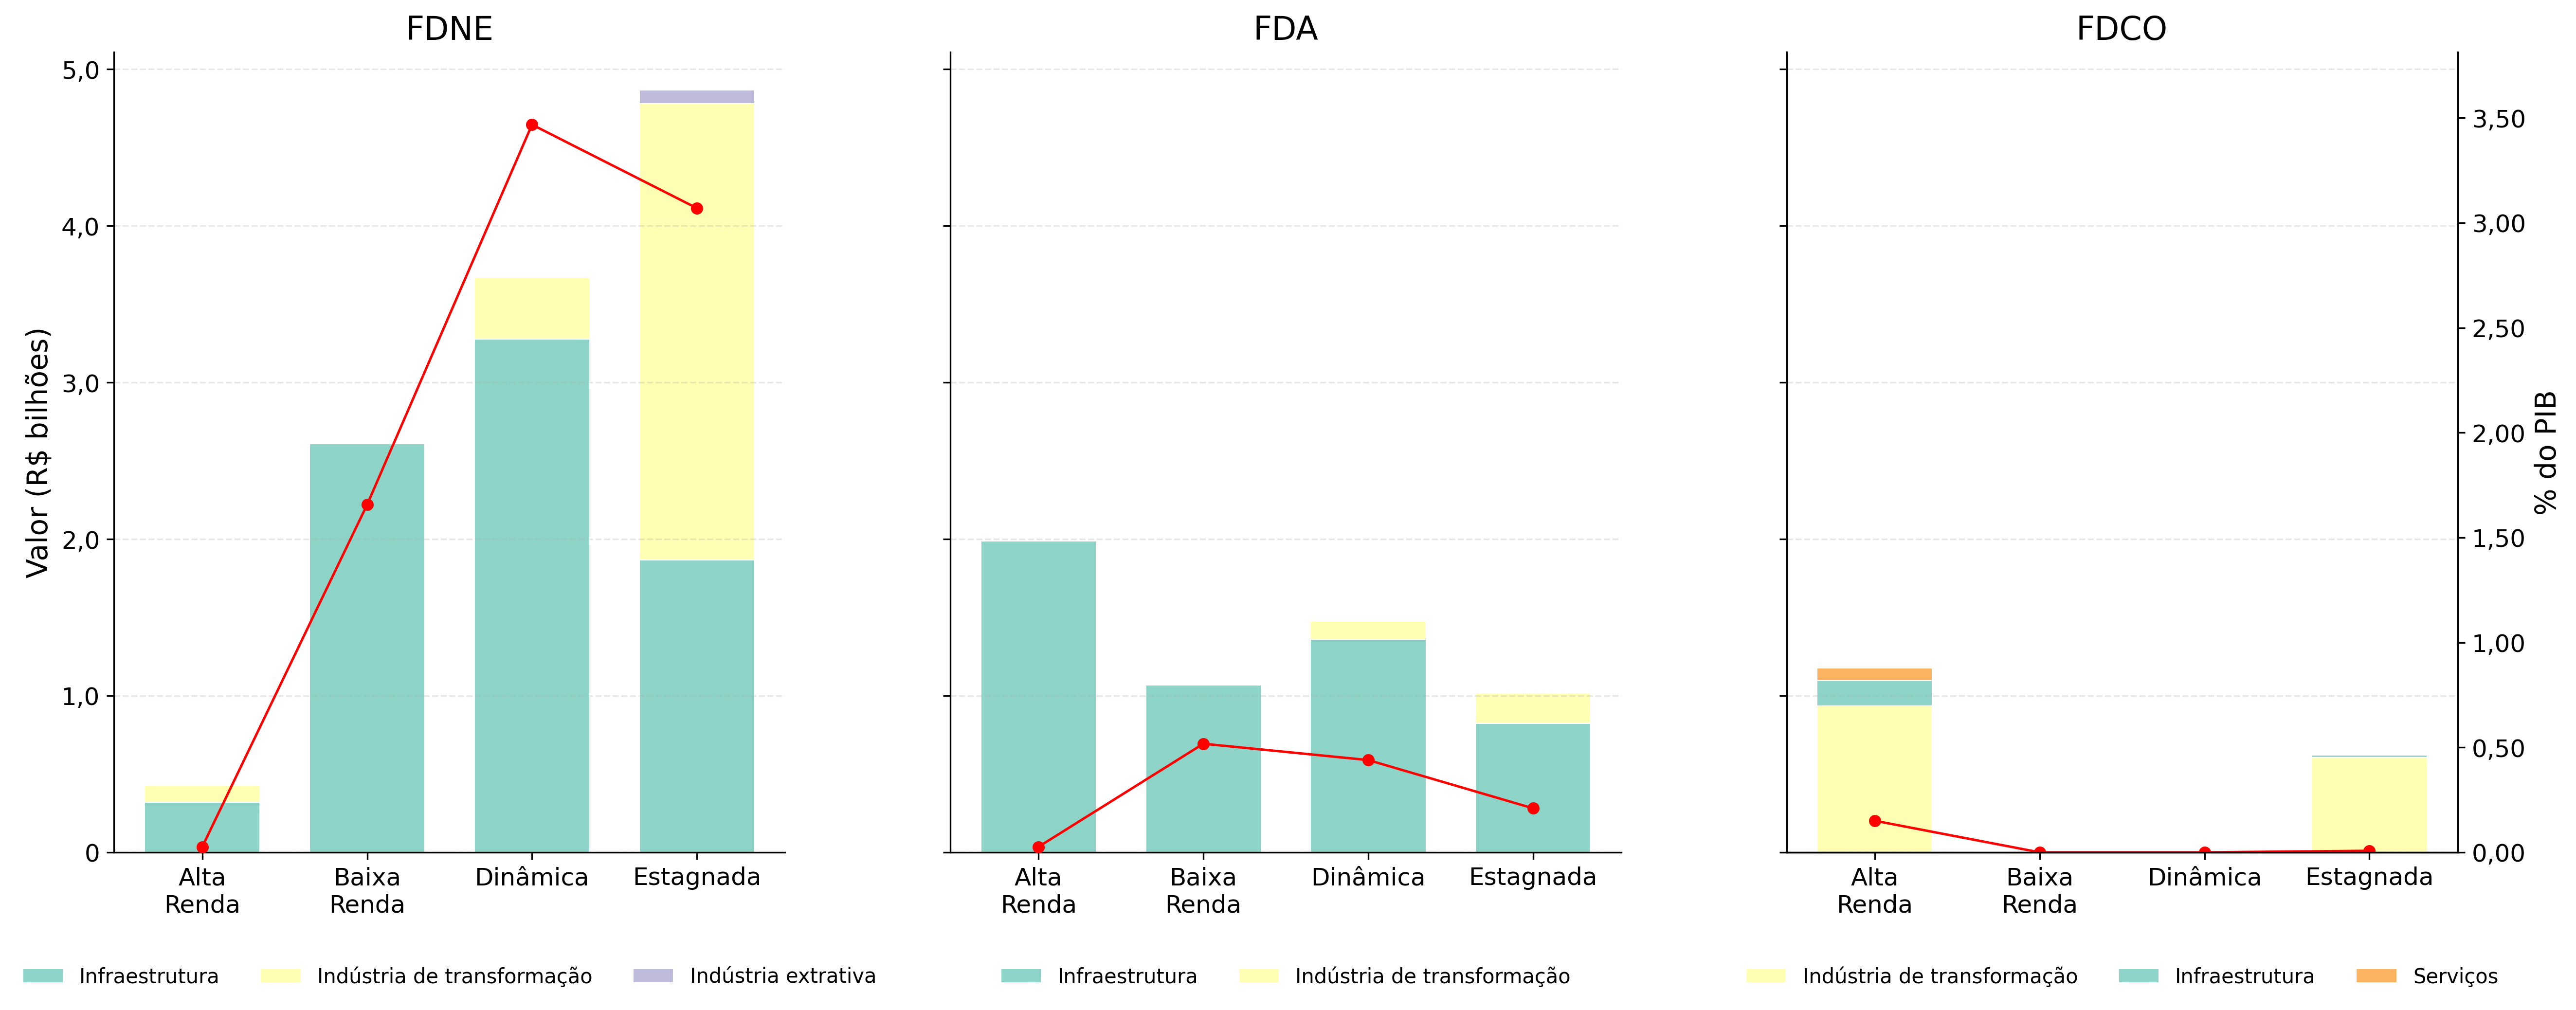
\includegraphics[width=1\textwidth]{fd_fundo_setor.png}
	\fonte{Elaborada pelos autores.}
\end{figure}

\subsection{Incentivos Fiscais}
\label{subsec:ifs}

Os Incentivos Fiscais são os instrumentos de desenvolvimento regional mais longevos, tendo sido promulgados pela Lei nº 4.069/1962 no âmbito da Amazônia Legal e pela Lei nº 4.239/1963 na região Nordeste, estabelecendo redução ou isenção de IR às empresas instaladas nessas regiões. Diferentemente dos Fundos Constitucionais e dos Fundos de Desenvolvimento, que envolvem financiamento direto, os Incentivos Fiscais operam por meio de renúncia tributária, ou seja, redução da carga de impostos devidos pelas empresas beneficiadas. Em 1997, a Lei nº 9.532/1997 estipulou a diminuição gradativa do percentual de redução fiscal até sua completa extinção em 2013. Porém, a Medida Provisória nº 2.199-14/2001 revogou a regulamentação anterior e estabeleceu uma redução fixa de 75\% do IRPJ para empresas beneficiadas, inicialmente válida até 2018, posteriormente postergada até 2023 e, recentemente, estendida até 2028 pela Lei nº 14.753/2023.

Segundo \citeonline{Shirasu2023} e \citeonline{Portugal2024}, a hipótese subjacente ao programa é que a redução do custo tributário gera incentivos para empresas investirem e se instalarem em regiões de menor desenvolvimento, atuando sobre o custo de oportunidade do capital e tornando mais atrativo investir nas regiões beneficiadas. São elegíveis aos benefícios os projetos de instalação, ampliação, modernização ou diversificação de linhas de produção de empresas enquadradas em setores classificados como prioritários para o desenvolvimento regional nas áreas de atuação da SUDENE e SUDAM. Porém, \citeonline{Portugal2024} aponta que há uma desvinculação dos Incentivos Fiscais em relação aos objetivos do desenvolvimento regional e defende uma redefinição completa do programa, argumentando que a definição dos setores prioritários é prerrogativa do presidente da República (Decreto nº 4.212/2002), apesar da existência dos planos regionais de desenvolvimento elaborados em discussão com a sociedade.

Em 2021, as renúncias de IRPJ decorrentes dos incentivos da SUDAM somaram cerca de R\$ 12,6 bilhões, sendo R\$ 9,7 bilhões ligados à indústria e R\$ 2,8 bilhões à agricultura\footnote{Demonstrativos dos Gastos Tributários (DGT), publicados pela Receita Federal do Brasil.}. No âmbito da SUDENE, o montante alcançou R\$ 19,3 bilhões, sendo R\$ 14,9 bilhões destinados à indústria e R\$ 4,4 bilhões à agricultura. Em um período mais longo, de 2015 a 2024, os dois programas de incentivo fiscal respondem por R\$ 126 bilhões em gastos tributários. A Figura~\ref{fig:incentivos} apresenta a distribuição dos benefícios por superintendência, setor e tipologia municipal.

% Gerado por: scripts/generate_policy_figures.py
\begin{figure}[htbp]
	\centering
	\caption{Distribuição dos incentivos fiscais, por superintendência, tipologia municipal e setor de atividade (2010-2021)}
	\label{fig:incentivos}
	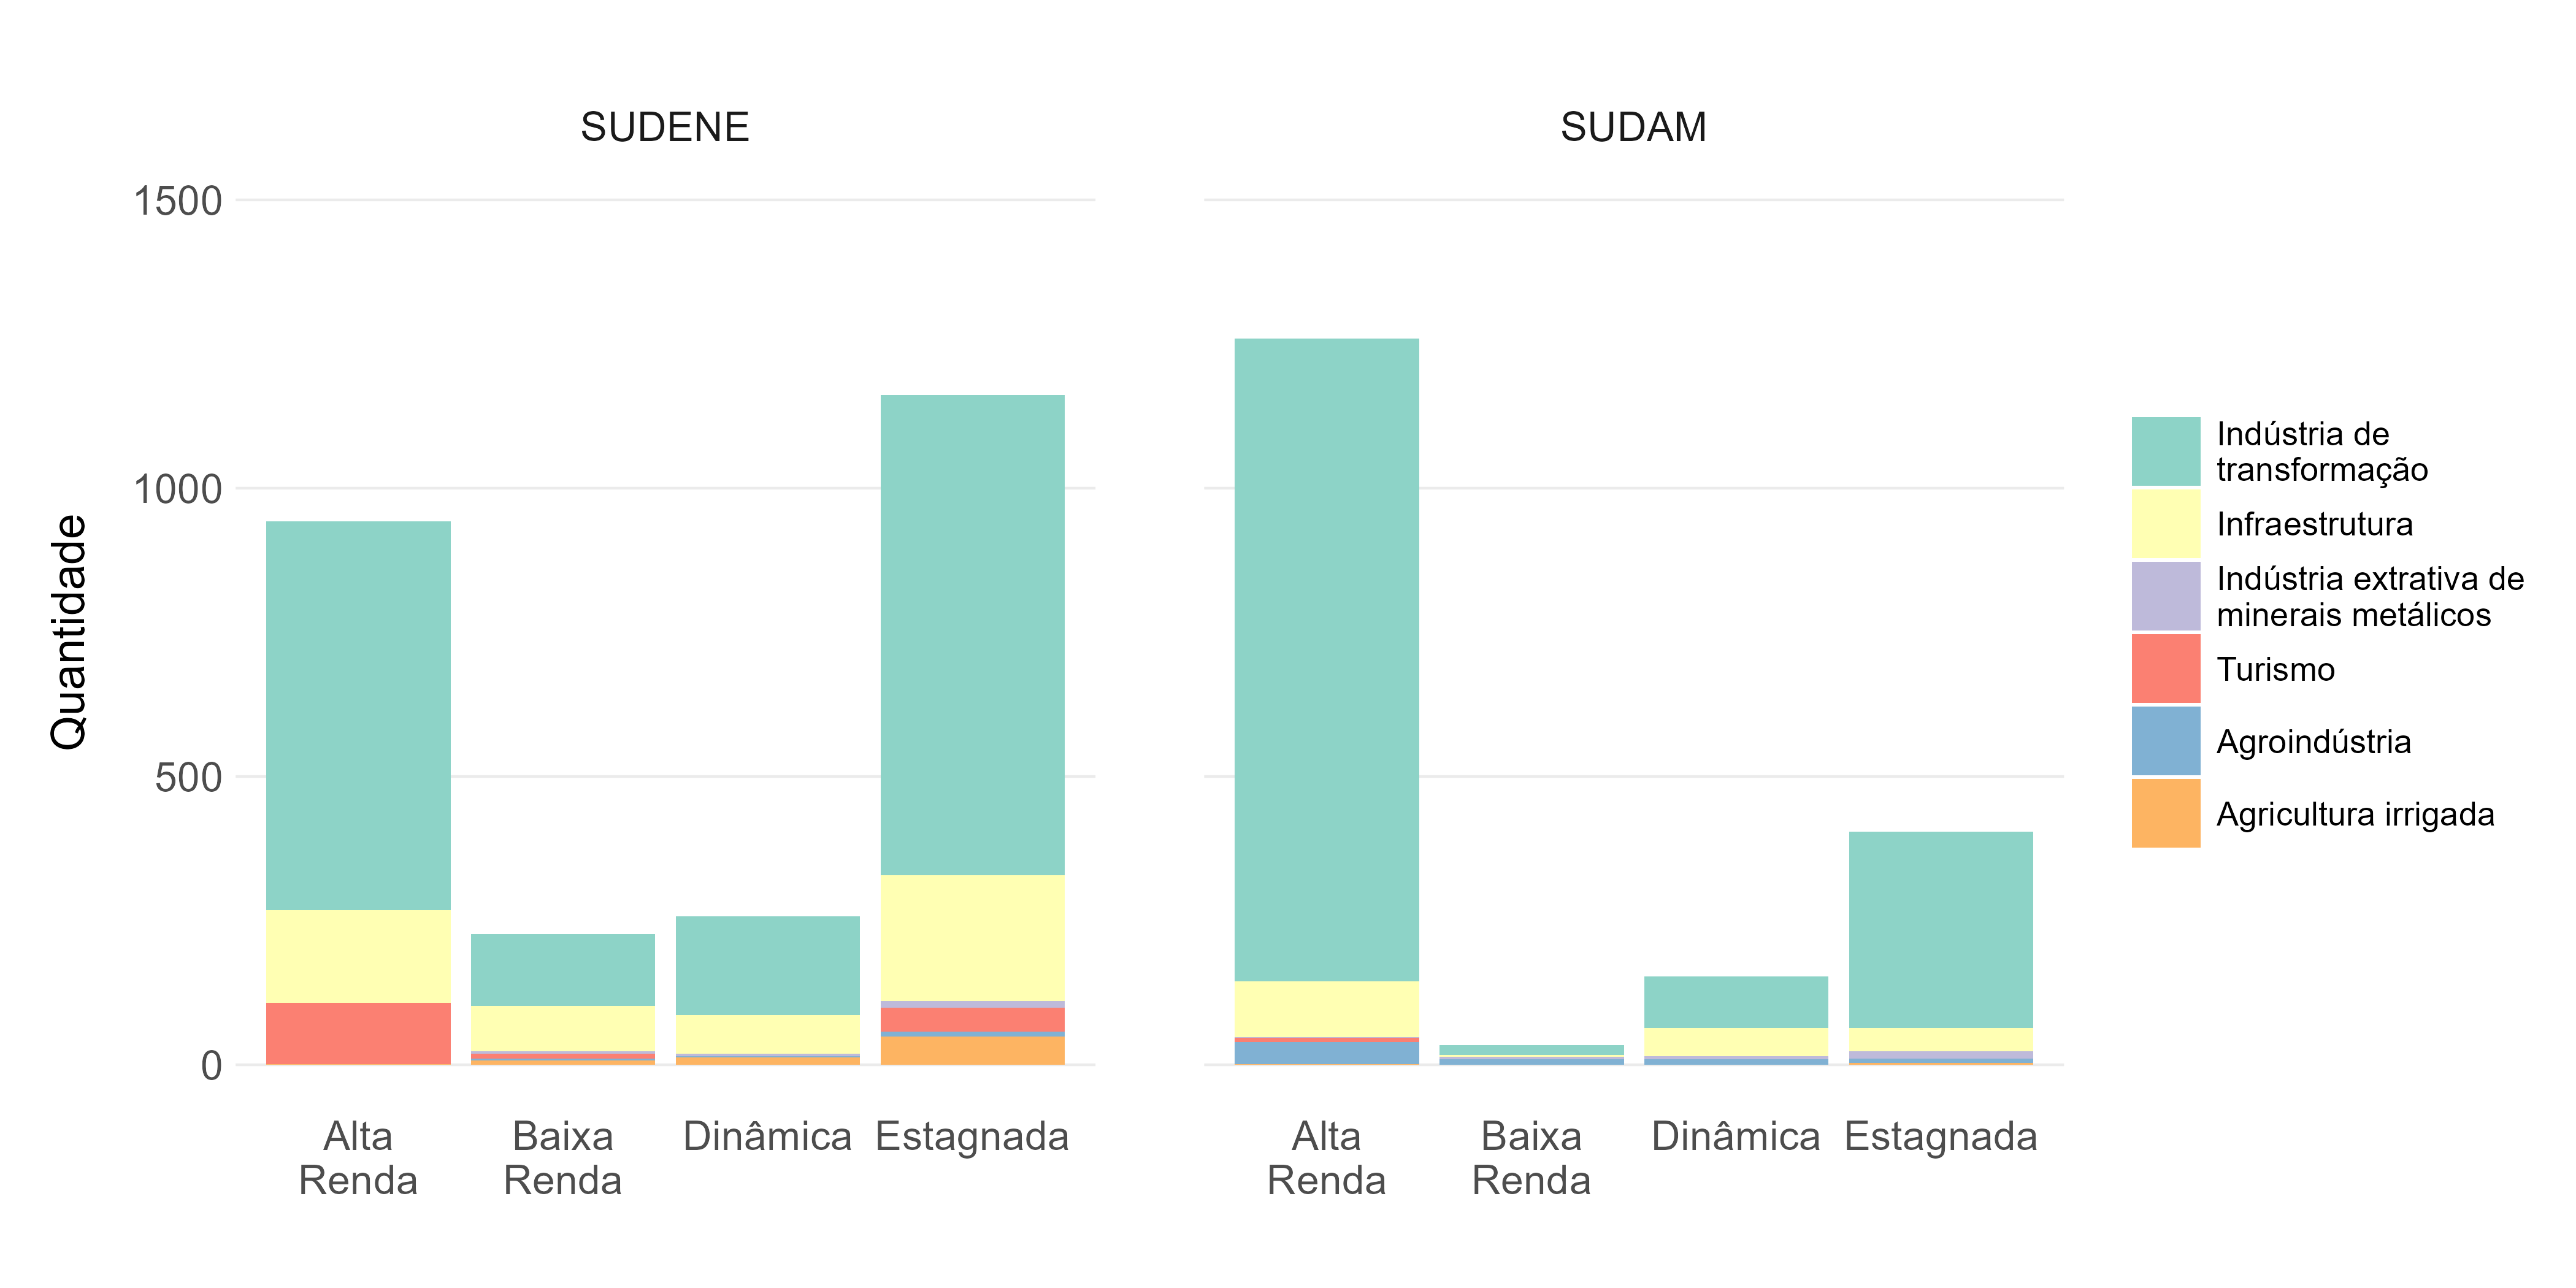
\includegraphics[width=1\textwidth]{icf_superint_setor.png}
	\fonte{Elaborada pelos autores.}
\end{figure}

No período de 2010 a 2021, SUDAM e SUDENE apoiaram 1.851 e 2.590 empresas com Incentivos Fiscais, respectivamente \cite{Portugal2024}. Os projetos da SUDAM apresentam alta concentração em municípios de alta renda, com 1.260 empresas, contra apenas 34 em municípios de baixa renda. Na SUDENE, os incentivos se distribuem de forma mais equilibrada, com prevalência de projetos em regiões estagnadas (1.162), frente a regiões de alta renda (943). Em termos setoriais, os projetos são majoritariamente ligados à indústria de transformação, com cerca de 76\% do total, e à infraestrutura (16\%), distribuição que se repete em nível de superintendência e tipologia.

Em síntese, a estrutura vigente de instrumentos da PNDR combina três mecanismos complementares de intervenção: os Fundos Constitucionais, voltados ao crédito subsidiado de ampla capilaridade territorial e com foco preferencial em micro e pequenos produtores; os Fundos de Desenvolvimento, direcionados a projetos estruturantes de grande porte; e os Incentivos Fiscais, que operam via redução da carga tributária para atrair investimentos privados às regiões prioritárias. Embora compartilhem o objetivo de promover o desenvolvimento das regiões menos dinâmicas, os instrumentos diferem substancialmente em volume de recursos, público-alvo, mecanismo de operação e grau de aderência aos objetivos da política \cite{Portugal2020, Portugal2024}.

Essa diversidade institucional, somada à persistência das desigualdades regionais que motivam a intervenção estatal, torna imprescindível a avaliação rigorosa dos efeitos de cada instrumento sobre os indicadores socioeconômicos locais. A literatura empírica tem buscado enfrentar essa tarefa com crescente sofisticação metodológica, e sua síntese constitui o objeto da revisão sistemática apresentada neste artigo.


\section{Método}
\label{sec:metodo}
\input{3-metodo}

\input{4-resultados}

\section{Considerações Finais}
\label{sec:consideracoes}
% Arquivo: latex/5-consideracoes.tex
% Seção 5: Considerações Finais

Esta revisão sistemática mapeou 34 estudos empíricos que avaliam os efeitos dos instrumentos da PNDR sobre indicadores socioeconômicos locais, cobrindo o período de 2005 a 2026. A análise do conjunto de evidências permite identificar cinco achados transversais.

Primeiro, há expressiva assimetria no volume de evidências entre instrumentos. Os Fundos Constitucionais concentram 28 dos 34 estudos, com predominância do FNE (24 estudos), enquanto os Fundos de Desenvolvimento (8 estudos) e os Incentivos Fiscais (9 estudos) permanecem substancialmente menos investigados. Essa desproporção é particularmente relevante dado o volume fiscal dos instrumentos menos avaliados: os Incentivos Fiscais da SUDAM e SUDENE totalizaram R\$ 126 bilhões em gastos tributários no período 2015--2024, sem que haja avaliações dedicadas aos incentivos da SUDAM ou análises de custo-efetividade de qualquer dos programas.

Segundo, os efeitos sobre o mercado de trabalho apresentam maior convergência entre os estudos do que os efeitos sobre o PIB \textit{per capita}. Para o emprego formal, há evidências consistentes de impacto positivo do FNE, com magnitude crescente nos primeiros anos pós-tratamento e efeitos mais pronunciados em micro e pequenas empresas e na modalidade de crédito para investimento. Para o PIB \textit{per capita}, os resultados são heterogêneos e fortemente condicionados à especificação econométrica, ao período amostral e à escala geográfica. Essa divergência sugere que os instrumentos podem ser mais eficazes na geração de postos de trabalho do que na elevação sustentada da renda média local.

Terceiro, a eficácia dos Fundos Constitucionais sobre o produto é condicionada ao nível inicial de renda dos municípios. Efeitos positivos concentram-se em faixas intermediárias de desenvolvimento, são nulos ou inconclusivos em municípios de baixa renda e decrescentes em municípios de alta renda. Esse padrão é consistente com a hipótese de capacidade de absorção: municípios mais pobres podem carecer do capital humano e da infraestrutura necessários para converter crédito subsidiado em crescimento sustentado, enquanto municípios de renda intermediária possuem o mínimo de condições para ativar o efeito multiplicador dos investimentos.

Quarto, os Fundos de Desenvolvimento apresentam indícios de impacto expressivo sobre o PIB \textit{per capita} --- entre 19\% e 24\% ---, com presença de efeitos de transbordamento espacial para municípios vizinhos. Esses valores são consideravelmente superiores aos estimados para os Fundos Constitucionais, o que pode refletir a escala dos empreendimentos financiados e sua concentração em infraestrutura e indústria de transformação. A base empírica, contudo, restringe-se a estudos recentes (2024--2026) com metodologias semelhantes e períodos parcialmente sobrepostos.

Quinto, a variável salário médio não apresenta variação significativa na maioria das avaliações dos instrumentos federais, indicando que novos postos de trabalho são criados ao nível salarial vigente, sem ganhos adicionais de produtividade. No âmbito estadual, a avaliação do Prodepe (PE) aponta redução salarial concomitante ao aumento do emprego, suscitando preocupação sobre a qualidade dos postos gerados por incentivos subnacionais.

Esses achados têm implicações para o desenho da política regional. A constatação de que crédito subsidiado é insuficiente para dinamizar municípios de baixa renda sugere a necessidade de complementaridade com investimentos em infraestrutura, capital humano e capacidades institucionais locais --- condições prévias à eficácia do instrumento. A ausência de ganhos salariais associados à geração de empregos indica que os instrumentos, em sua configuração atual, tendem a expandir a atividade econômica sem transformar a estrutura produtiva. A concentração dos Incentivos Fiscais em municípios de maior dinamismo, documentada na literatura, contrasta com o objetivo redistributivo da PNDR e aponta para a necessidade de revisão dos critérios de concessão.

Do ponto de vista metodológico, este artigo constitui a primeira revisão sistemática dedicada aos instrumentos de financiamento da PNDR. A estratégia de busca abrangeu cinco bases de dados acadêmicas, a classificação dos registros empregou modelo de linguagem de grande escala com revisão humana integral, a seleção dos estudos foi respaldada por índice de citação cruzada --- que permitiu justificar a inclusão de literatura cinzenta com base em reconhecimento pela própria comunidade acadêmica --- e a deduplicação percorreu quatro fases complementares (DOI exato, similaridade de título, identidade de PDF e verificação manual de textos para discussão e versões de congresso).

Não obstante, o estudo possui limitações que devem ser explicitadas. A heterogeneidade de métricas, períodos amostrais e especificações econométricas entre os estudos primários inviabiliza a condução de meta-análise formal, restringindo a síntese ao plano qualitativo. Os resultados desta revisão dependem, ademais, da qualidade e da comparabilidade dos trabalhos incluídos, cujas estratégias de identificação causal variam substancialmente em robustez. Embora a inclusão de literatura cinzenta atenue o risco de viés de publicação, tal risco não pode ser inteiramente eliminado. A triagem assistida por modelo de linguagem demandou correção em dois terços dos registros classificados, o que evidencia a necessidade de validação integral pelo pesquisador e impede a delegação autônoma dessa etapa. Por fim, a busca restringiu-se a cinco bases de dados, de modo que estudos indexados exclusivamente em outros repositórios podem não ter sido capturados.

Do ponto de vista da agenda de pesquisa, três prioridades emergem desta revisão: (i)~a ampliação das evidências sobre Fundos de Desenvolvimento --- especialmente FDA e FDCO, para os quais inexistem avaliações quantitativas dedicadas --- e sobre os Incentivos Fiscais da SUDAM; (ii)~a condução de estudos que avaliem simultaneamente os três instrumentos e suas interações, dado que a quase totalidade das avaliações examina cada instrumento isoladamente, sem capturar possíveis sinergias ou redundâncias; e (iii)~a adoção de desenhos quase experimentais com maior poder de identificação causal --- como regressão com descontinuidade e controle sintético ---, que permanecem sub-representados na literatura frente a métodos com maior fragilidade na separação do efeito da política de fatores confundidores.


% =============================================================================
% REFERENCES
% =============================================================================
\bibliographystyle{abntex2-alf}
\bibliography{references}

\end{document}
